%(BEGIN_QUESTION)
% Copyright 2006, Tony R. Kuphaldt, released under the Creative Commons Attribution License (v 1.0)
% This means you may do almost anything with this work of mine, so long as you give me proper credit

Beregn spenningsfallene i denne sløyfematede 4-20 mA-senderkretsen for strømforholdene i tabellen:

$$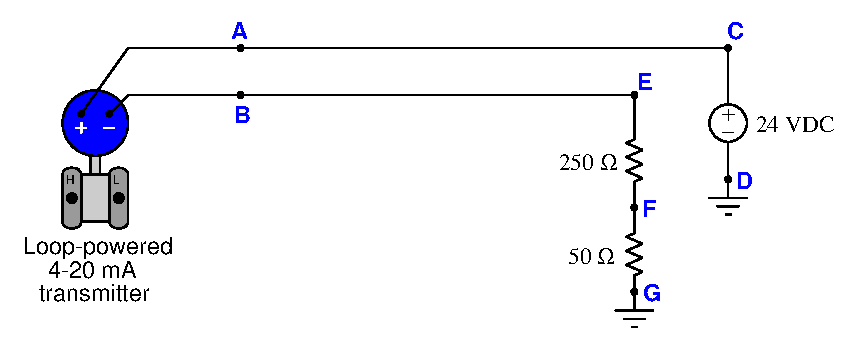
\includegraphics[width=15.5cm]{i00129x01.eps}$$

% No blank lines allowed between lines of an \halign structure!
% I use comments (%) instead, so that TeX doesn't choke.

$$\vbox{\offinterlineskip
\halign{\strut
\vrule \quad\hfil # \ \hfil & 
\vrule \quad\hfil # \ \hfil & 
\vrule \quad\hfil # \ \hfil & 
\vrule \quad\hfil # \ \hfil & 
\vrule \quad\hfil # \ \hfil & 
\vrule \quad\hfil # \ \hfil \vrule \cr
\noalign{\hrule}
%
% First row
Prosent av område & Senderstrøm & $V_{CD}$ & $V_{EF}$ & $V_{FG}$ & $V_{AB}$ \cr
%
\noalign{\hrule}
%
% Another row
0 \% & 4 mA &  &  &  &  \cr
%
\noalign{\hrule}
%
% Another row
25 \% & 8 mA &  &  &  &  \cr
%
\noalign{\hrule}
%
% Another row
50 \% & 12 mA &  &  &  &  \cr
%
\noalign{\hrule}
%
% Another row
75 \% & 16 mA &  &  &  &  \cr
%
\noalign{\hrule}
%
% Another row
100 \% & 20 mA &  &  &  &  \cr
%
\noalign{\hrule}
} % End of \halign 
}$$ % End of \vbox

For at en sløyfematet sender skal fungere korrekt, må det til enhver tid være en minimum DC-spenning over terminalene ($V_{AB}$). Typisk verdi er 12 volt (merk at minimumsverdien varierer mellom produsenter og modeller). Angi hvilke sløyfeforhold som kan true denne minimumsspenningen, og hvordan du som tekniker vil sikre at senderen alltid får tilstrekkelig spenning.

\vskip 20pt \vbox{\hrule \hbox{\strut \vrule{} {\bf Forslag til sokratisk diskusjon} \vrule} \hrule}

\begin{itemize}
\item{} Hvis en tekniker måler senderspenningen samtidig som trykket på «H»-porten plutselig øker, vil den målte spenningen øke eller synke?
\item{} Kretsen viser {\it to} motstander, ikke bare én. Hva er en praktisk grunn til at en 4-20 mA-sløyfe kan inneholde flere motstander?
\item{} Vis hvordan man kan {\it estimere} numeriske svar på oppgaven uten kalkulator.
\end{itemize}

\underbar{file i00129}
%(END_QUESTION)





%(BEGIN_ANSWER)

% No blank lines allowed between lines of an \halign structure!
% I use comments (%) instead, so that TeX doesn't choke.

$$\vbox{\offinterlineskip
\halign{\strut
\vrule \quad\hfil # \ \hfil & 
\vrule \quad\hfil # \ \hfil & 
\vrule \quad\hfil # \ \hfil & 
\vrule \quad\hfil # \ \hfil & 
\vrule \quad\hfil # \ \hfil & 
\vrule \quad\hfil # \ \hfil \vrule \cr
\noalign{\hrule}
%
% First row
Prosent av område & Senderstrøm & $V_{CD}$ & $V_{EF}$ & $V_{FG}$ & $V_{AB}$ \cr
%
\noalign{\hrule}
%
% Another row
0 \% & 4 mA & 24 V & 1 V & 0.2 V & 22.8 V \cr
%
\noalign{\hrule}
%
% Another row
25 \% & 8 mA & 24 V & 2 V & 0.4 V & 21.6 V \cr
%
\noalign{\hrule}
%
% Another row
50 \% & 12 mA & 24 V & 3 V & 0.6 V & 20.4 V \cr
%
\noalign{\hrule}
%
% Another row
75 \% & 16 mA & 24 V & 4 V & 0.8 V & 19.2 V \cr
%
\noalign{\hrule}
%
% Another row
100 \% & 20 mA & 24 V & 5 V & 1 V & 18 V \cr
%
\noalign{\hrule}
} % End of \halign 
}$$ % End of \vbox

Rosemount 3144-temperatursenderen krever for eksempel minimum 12 volt over terminalene for analog drift, og 18.1 volt for korrekt drift under HART-kommunikasjon (digitalt over analogt signal). Merk hvordan drift av en slik 3144-sender i en sløyfe med 24 V forsyning og 300 ohm total motstand kan bli kritisk nær toppen av signalområdet.

%(END_ANSWER)





%(BEGIN_NOTES)


%INDEX% Basics, loop-powered transmitter: voltage drop calculations

%(END_NOTES)
